\documentclass[a4paper,10pt]{article} 

\usepackage[utf8]{inputenc} 
%\usepackage[T1]{fontenc}

\usepackage{textcomp}           % Extra Symbole (Grad Celsius etc.)
\usepackage{amssymb,amsmath}    % Schöne Formeln (AMS = American Mathematical Society)
\usepackage{graphicx}           % Bilder und Seitenränder
\usepackage{subcaption}			% captions for subfigures
\usepackage{booktabs}           % Schönere Tabellen
\usepackage{colortbl}           % Farbige Tabellen

%\usepackage{tcolorbox}			% schöne bunte Boxen
\usepackage{mathtools}			% \mathclap für ordentliche \underbrace-			environments
\usepackage{geometry}			% Pagelayout mit \newgeometry, \restoregeometry
\usepackage{float}
\usepackage{wrapfig}
\usepackage{enumitem}
\usepackage{float}
\usepackage{braket}
\usepackage{caption}
\input{insbox.tex}
%\usepackage{pst-optexp}
%\usepackage{auto-pst-pdf}

\graphicspath{{./img/}}


\bibliographystyle{unsrtnat}

\renewcommand{\k}{\mathbf{k}}
\begin{document}
\begin{titlepage}
 \begin{center}
	\Large{Advanced laboratory class 2}
	\end{center}
	\begin{center}
	 \LARGE{\textbf{FP2 - Digital holography}}
	\end{center}
	
	\begin{center}
	
	\large Marco \textsc{Canteri} \\
	marco.canteri@student.uibk.ac.at
	\end{center}
	
	\begin{center}
	\vspace{1cm}
	Innsbruck, \today
	\vspace{2cm}
	\end{center}
	
	\begin{center}
	
\includegraphics[scale=0.4]{img/uibk} 
	\end{center}

\end{titlepage}
\begin{abstract}
In this experiment we studied a device called spatial light modulator (SLM). First we created a blazed grating with the SLM, this allowed us to measure the pixel size of our SLM which we found to be $7.94\pm 0.01 \, \mu \text{m}$. Then we also used the SLM to simulate a diffraction lens, to reproduce two points on a screen, and to draw more complex images using the Gerchberg-Saxton algorithm. Lastly, we studied how the SLM can be exploited for adaptive optic applications.
\end{abstract}
\section{Introduction}
Holograms are a particular phase and amplitude distribution of a light field that can be stored. Such distribution could be, for example, the light scattered by a real object which is illuminated with a reference wave. Another possibility is to use a spatial light modulator (SLM), this device can change the amplitude or the phase of a light field. Therefore it is possible to use it to create synthetic holograms. This is exactly what we did in this experiment. We used an SLM to create arbitrary images on a screen. First we displayed easier images such as points, then we also created more complex holograms with the Gerchberg-Saxton algorithm. Moreover, an SLM can be used to replicate diffraction lens, so it was possible to change the focus length of a lens. More important SLM are used in adaptive optics applications which are used to reduce distortion of an optical signal and correct it. This technology is widely used is many areas of science such as astronomy and microscopy.
\section{Theory}
\subsection{Spatial light modulator}
A spatial light modulator is basically a display which can be controlled by a computer. It is composed of a grid of pixels which usually contain birefringent molecules. Every pixel of the SLM can be controlled individually by applying a voltage to its ends, this causes a rearrangement of the molecules, so when the light field pass through the molecules it acquires a phase which depends on the molecules orientation. Therefore, it is possible to change the phase distribution of the light that goes through the SLM. SLM can also work on reflection mode, which means that the light does not pass through but it is reflected. As already mentioned, the SLM is controlled by a computer, it is like a second monitor where you can display an image which is then is converted in a phase pattern. Hence, to create an hologram with an SLM you must first understand which phase pattern is necessary. Usually the output light of the SLM is focused on a screen with a lens, so in this case the field of the SLM $E_S$ and the field on the screen $E_T$ are related via a Fourier transform 
\begin{equation}E_T(x,y) \propto \int E_S(x,y)e^{-i\frac{2\pi}{\lambda f}(ux+vy)}\,dudv,\end{equation}
where $\lambda$ is the wavelength of the light, and $f$ the focal length of the lens. To obtain the desired $E_T$, the electric field of the SLM can be found anti-transforming $E_T$, i.e.
\begin{equation}\label{slmdistribution}
E_S(u,v) \propto \int E_T(x,y)e^{i\frac{2\pi}{\lambda f}(ux+vy)}\,dxdy.
\end{equation}
Usually it is mathematically complicated to calculate such anti-transformation, so, even if there are analytical solutions in some cases, in most cases it is necessary to calculate approximated solution. In the next two sections we will see an example of an analytical solution and a general algorithm that can be used to obtain $E_S$ from an arbitrary $E_T$.
\subsection{Blazed grating}\label{blazedsection}
The simplest intesity distribution $E_T$ is a single point on the screen. Mathematically it can be described with Dirac deltas
\begin{equation}E_T(u,v) = \delta(x-x_0)\delta(y-y_0),\end{equation}
where $(x_0,y_0)$ is the position of the point. $E_S$ can be calculated with equation \eqref{slmdistribution}, the integration is straightforward due to the deltas
\begin{equation}E_S(u,v) \propto \int \delta(x-x_0)\delta(y-y_0)e^{i\frac{2\pi}{\lambda f}(ux+vy)}\,dxdy = e^{i\frac{2\pi}{\lambda f}(ux_0+vy_0)}.\end{equation}
Therefore to create a point distribution, the field of the SLM must have a phase of $\phi(u,v) = \frac{2\pi}{\lambda f}(ux_0+vy_0) \mod 2\pi$. This particular phase distribution is called blazed grating, it can be seen in figure \ref{blazed}.\\
The period of the grating $d$ is related with the angle $\alpha$ between the peak relative to the 0th order and the 1st one by \cite{grating}
\begin{equation}d\sin \alpha = \lambda.\end{equation}
The angle $\alpha$ can be expressed with the distance $x_i$ between the already mentioned peaks as follows \cite{skriptum}
\begin{equation}\alpha =\arctan\left(\frac{x_i}{f}\right).\end{equation}
Therefore the the grating period can be written as
\begin{equation}\label{gratingperiod} d = \frac{\lambda}{\sin\left(\arctan\left(\frac{x_i}{f}\right)\right)}.\end{equation}
In conclusion it is possible to find the pixel size of the SLM by measuring the distance $x_i$ and knowing the value of $d$ in unit of pixel, then the pixel size is the ratio between $d$ calculated with equation \eqref{gratingperiod} and its value in pixel.\\
\begin{figure}[H]
\centering
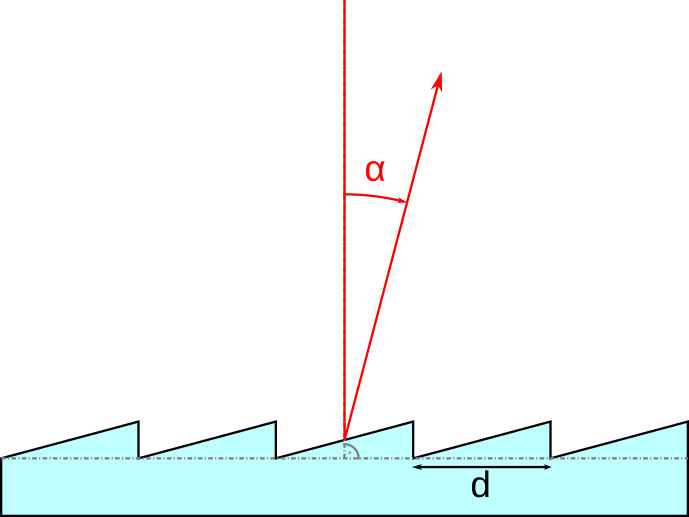
\includegraphics[width=0.5\textwidth]{blazed}
\caption{Blazed grating with period $d$, $\alpha$ is the first order diffraction angle }\label{blazed}
\end{figure}
\subsection{Gerchberg-Saxton algorithm}
Equation \eqref{slmdistribution} cannot be always solved analytically, so it is necessary to use an algorithm to find an approximated solution. This can be done with the Gerchberg-Saxton algorithm \cite{algorithm}. This algorithm works through iterations: first a guess of the needed phase distribution is made, this guess is propagated to the image plan. The phase of this distribution along with the desired intensity distribution is used to calculate the right initial guess, the resulting phase distribution of this step is used to for the next iteration. A scheme of this algorithm is in figure \ref{gs} 
\begin{figure}[H]
\centering
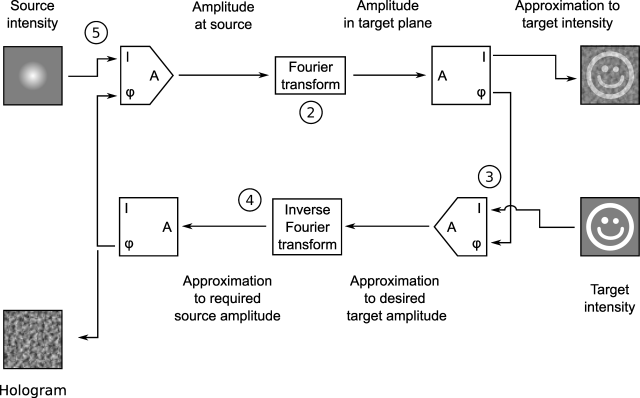
\includegraphics[width=0.7\textwidth]{GS-diagram}
\caption{Gerchberg-Saxton algorithm, the source intensity in our case is our laser and the hologram is the phase distribution on the SLM}\label{gs}
\end{figure}
\section{Experiment setup}\label{setupsection}
\begin{figure}[H]
\centering
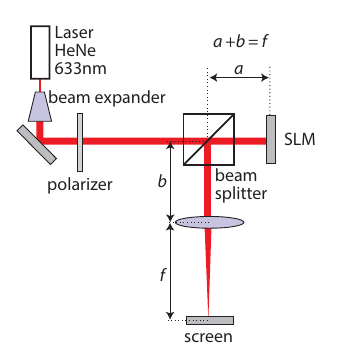
\includegraphics[width=0.5\textwidth]{setup1}
\caption{Experiment setup for the first part of the experiment}\label{setup1}
\end{figure}
The experiment setup is depicted in figure \ref{setup1}. The source is a Helium-Neon laser with wavelength of 633 nm. After the source, the beam is expanded such that it hits all the surface of the SLM. The SLM works in reflection mode, so the incoming and outgoing beam are separated with a beam splitter. Finally the beam is focused on a screen with a lens which has a focal length of 20 cm. The power of the beam was controlled with a polarizer placed after the beam expander. The screen is a camera mVBluefox-22-1G with a resolution of 1024x768 and a pixel size of 4.65 $\mu m$ \cite{camerasite}. The SLM has a resolution of 1920x1080 pixel and it is controlled with the graphic card of a computer and the software MATLAB. The camera is monitored with the computer as well.\\
For the last part of the experiment the setup was modified, it can be seen in figure \ref{setup2}. In order to perform some adaptive optic task, we built a interferometer. Another mirror was added after the beam splitter, and after the lens we placed an iris diaphragm to block every order but the first one. Lastly another lens with focal length 10 cm was used to focus the image on the camera.
\begin{figure}[H]
\centering
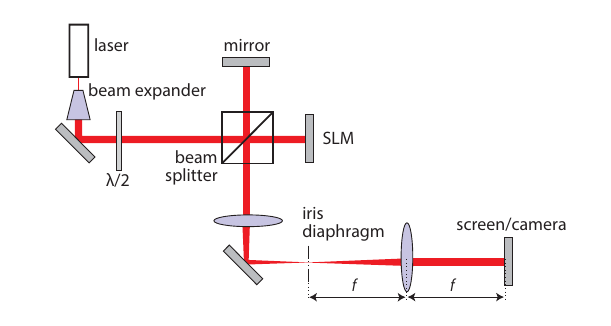
\includegraphics[width=0.7\textwidth]{setup2}
\caption{Experiment setup for the last part of the experiment}\label{setup2}
\end{figure}
\section{Experiment and Data analysis}
\subsection{Grating and SLM pixel size}
\begin{figure}[H]
\centering
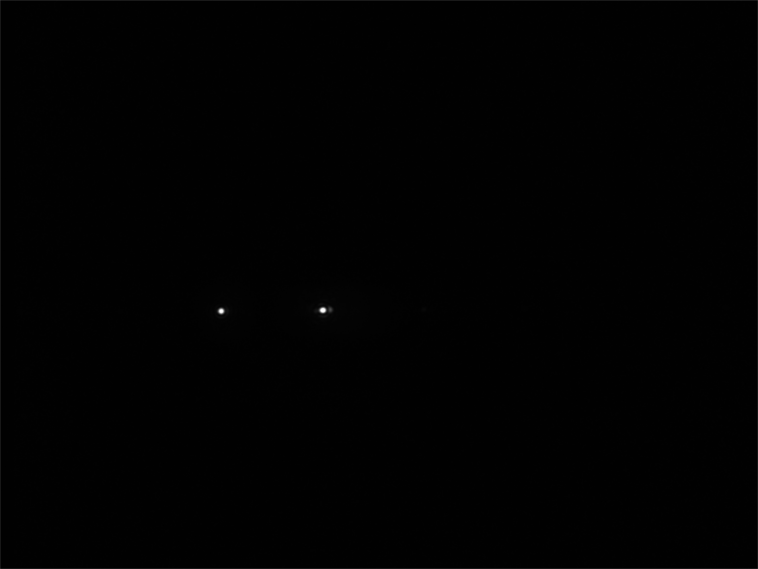
\includegraphics[width=0.5\textwidth]{intensity0}
\caption{Example of the acquired data, we can clearly see two peaks which are the zeroth and the first order for a grating period of 25 pixels}
\end{figure}
With a MATLAB script we displayed a blazed grating on the SLM with period of 25,40, and 60 pixels. We took the images of the created hologram and of the background. The images were taken with an exposure time of 2125 $\mu$s for the background and for the grating of 25 pixels, while for the rest of the measurements we used an exposure time of 565 $\mu$s. For the analysis we subtracted the background from the images and we measured the distance between the first order and the zeroth order peaks. This analysis was done with the software ImageJ. The distance was calculated by taking the number of pixels between the maximum of intensity and multiplying it by the pixel size of the camera. The error on the distance $\sigma x_i$ is based on the resolution of the camera, which is its pixel size. Hence, the error on the distance is twice the pixel size of the camera. With equation \eqref{gratingperiod} we calculated $d$ in unit of meters and then the pixel size of the SLM as described in section \ref{blazedsection}. The three results relative to the three different periods are in following table. The error $\sigma d$ in the pixel size is calculated through propagation on equation \eqref{gratingperiod} 
\begin{equation}\sigma d = \frac{f\lambda}{x_i^2\sqrt{\frac{x_i^2}{f^2}+1}}\sigma x_i.\end{equation}
\begin{table}[H]
\centering
\begin{tabular}{c|c|c}
 Grating period [px]& peaks distance [$\mu$m] & SLM pixel size [$\mu$m] \\
  \hline
  25 & $637.0\pm9.3$ & $7.95\pm0.12$ \\
  \hline
  40 & $399.9\pm 9.3$ & $7.91 \pm 0.18$ \\
  \hline
  60 & $265.05\pm 9.3 $ & $7.96 \pm 0.28$ \\
  \hline
\end{tabular}
\caption{Pixel size of the SLM calculated for different grating periods.}
\end{table}
We fitted these values with a constant function $y=a$ and we obtained a pixel size of $7.94\pm 0.01\,\mu$m.
\subsection{Diffractive lens}
An SLM can be also used to create a diffractive lens, the distribution to display on the SLM in this case is \cite{skriptum}
\begin{equation}E_S(u,v) = e^{i\frac{\pi}{\lambda f^2}(u^2+v^2)z},\end{equation}
where $z$ is the focus shift. \\
We tried this formula with two different $z$, 10 and 15 cm. For both $z$ we then measured with a meter the new focus point by moving the camera along the $z$-axis until the image was in focus. From our measurements we obtained respectively 10.5 and 16 cm. Both measurements are within one centimeter of the theoretical one. The difference could arise from different sources. First of all the focal point is not well defined experimentally, it is difficult to find the right distance at which the image is focused. The SLM has also an intrinsic focal shift which change the actual one. There are also some limits in the shift $z$ given by the sampling of the camera sensor which could lead to aliasing, we are thus limited by the Nyquist–Shannon theorem, if the camera is placed to far we will see Moire fringes.
\subsection{Multiple foci}
\begin{figure}[H]
\centering
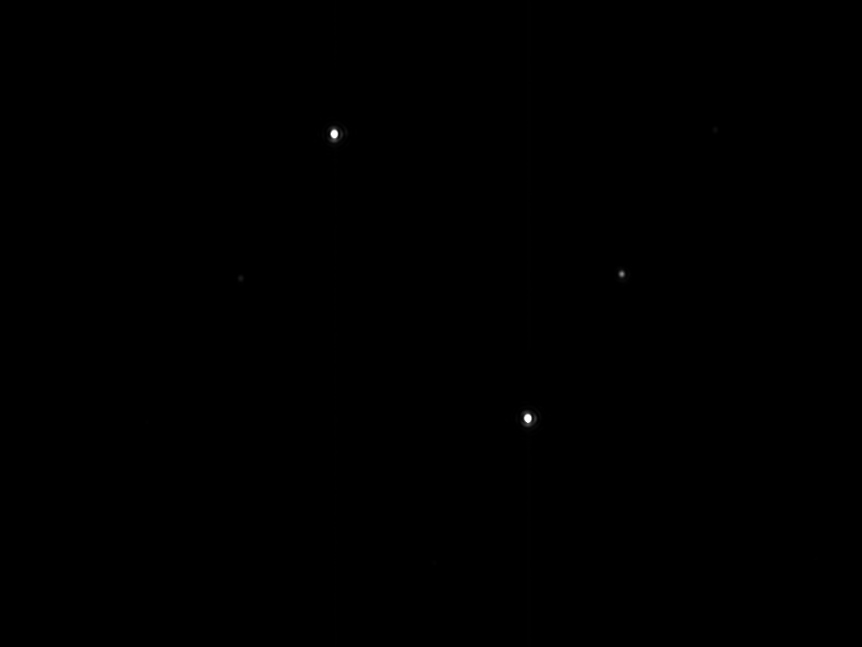
\includegraphics[width=0.5\textwidth]{combined}
\caption{Two points hologram created with the SLM, first orders are clearly visible, the zeroth orders which are less bright can be barely seen}\label{combined}
\end{figure}
We have already analyzed how we can display a single point on the screen. It is also possible to display more points with the SLM. The relation between the screen intensity and the phase distribution is by a Fourier transform. The point is transformed into a plane wave $e^{ikz}$, so, since the Fourier transform is linear, to display two points we need the sum of two different plane waves
\begin{equation}E_S = e^{ik_1 z} + e^{ik_2 z} = Ae^{i\phi}.\end{equation}
The sum of to complex numbers is of course a complex number, but since our SLM only changes the phase distribution, we must approximate our field leaving out the amplitude $A$. The amplitude could be changed with a two SLMs configuration. The phase we used is
\begin{equation}\phi = \text{Arg}(e^{i\phi_1} + e^{i \phi_2}),\end{equation}
where $\phi_1$ is the phase of a blazed grating with a period  of 50 pixels and $\phi_2$ is another blazed grating with period of 30 pixels. The resulting image is shown in figure \ref{combined}
\subsection{Gerchberg-Saxton algorithm}
\begin{figure}[H]
    \centering
    \begin{subfigure}[b]{0.49\textwidth}
        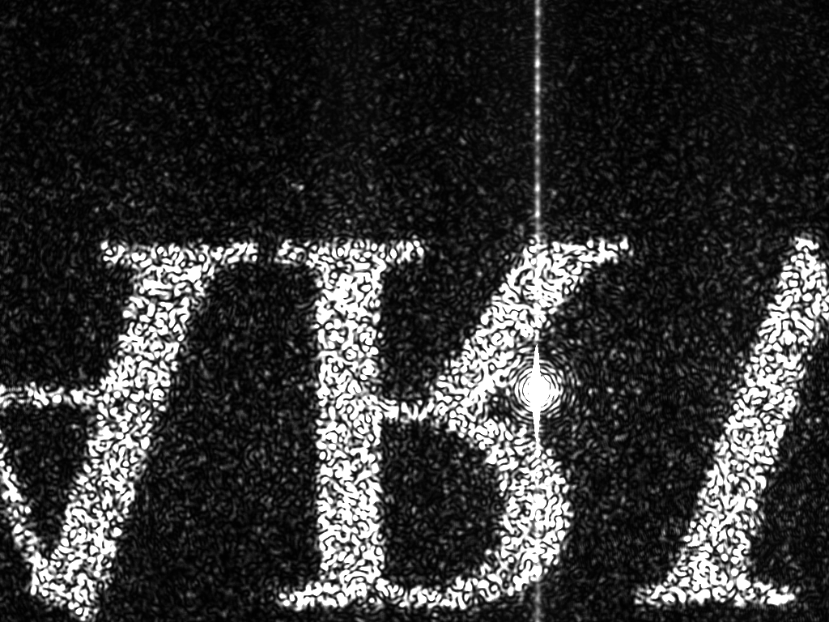
\includegraphics[width=\textwidth]{1iteration}
        \caption{Image after one iteration of the Gerchberg-Saxton algorithm}
    \end{subfigure}
    \hfill
    \begin{subfigure}[b]{0.49\textwidth}
        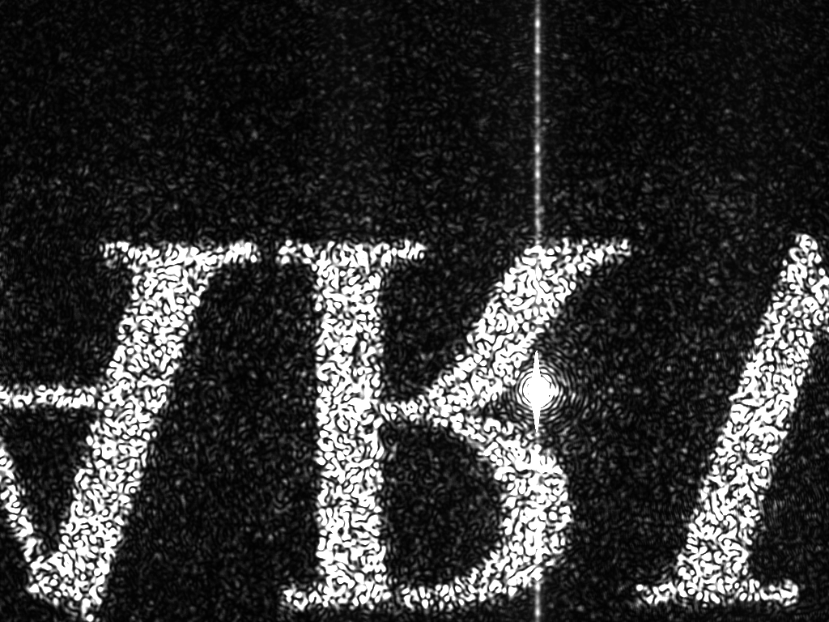
\includegraphics[width=\textwidth]{10iteration}
        \caption{Image after ten iteration of the Gerchberg-Saxton algorithm}
    \end{subfigure}
\caption{Images created with the Gerchberg-Saxton algorithm using a different number of iterations}\label{gsalgorithm}
\end{figure}
To test the Gerchberg-Saxton algorithm we used an arbitrary white and black image. We used the algorithm to calculate the phase distribution of the SLM and then we recorded the resulting images for different number of iterations. The result can be seen in figure \ref{gsalgorithm}. At first glance there is not a big difference, even with one iteration the algorithm does a good job to represent an arbitrary image. However a closer look reveals some details, the image with ten iterations has sharper edges, and the border between the black background and the white letters is more defined.
\section{Adaptive optics}
\begin{figure}[H]
    \centering
    \begin{subfigure}[b]{0.3\textwidth}
        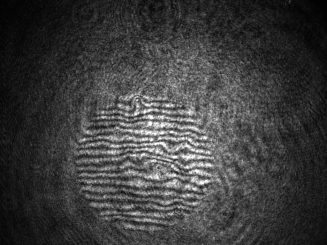
\includegraphics[width=\textwidth]{1pixel}
        \caption{Interference pattern with no shift in the grating}
    \end{subfigure}
    %
    \begin{subfigure}[b]{0.3\textwidth}
        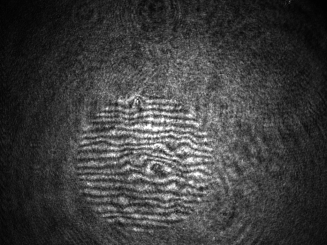
\includegraphics[width=\textwidth]{2pixel}
        \caption{Interference pattern with a shift of 1 pixel in the grating}
    \end{subfigure}
    %
    \begin{subfigure}[b]{0.3\textwidth}
        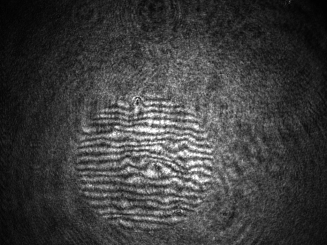
\includegraphics[width=\textwidth]{3pixel}
        \caption{Interference pattern with a shift of 2 pixels in the grating}
    \end{subfigure}
\caption{Interference patterns recorded}\label{interferencepatterns}
\end{figure}
For this last part of the experiment we changed setup as explained in section \ref{setupsection}. We placed in front of the SLM a piece of transparent tape, such that we can simulate an adaptive optic experiment, where a correction to the optical signal is applied in order to remove distortions, which in this case are caused by the tape. We then measured three different intensity distribution $I_1,I_2,I_3$. These distributions are obtained by shifting the grating on the SLM by respectively 0,1 and 2 pixels. The grating has a period of 3 pixels, so the phase shift gained by the shift in the grating is $2\pi/3$ for every shifted pixel. This measurements can be seen in figure \ref{interferencepatterns}.\\
The phase shift caused by the tape can be calculated as \cite{skriptum}
\begin{equation}\phi = \text{Arg}(I_1 + I_2 e^{i\frac{2\pi}{3}}+I_3 e^{i\frac{4\pi}{3}}.)\end{equation}
Therefore if the negative of this phase distribution is displayed on the SLM, it will cancel out the distortions introduced by the tape. The result of this correction is shown in figure \ref{corrected}

\begin{figure}[H]
\centering
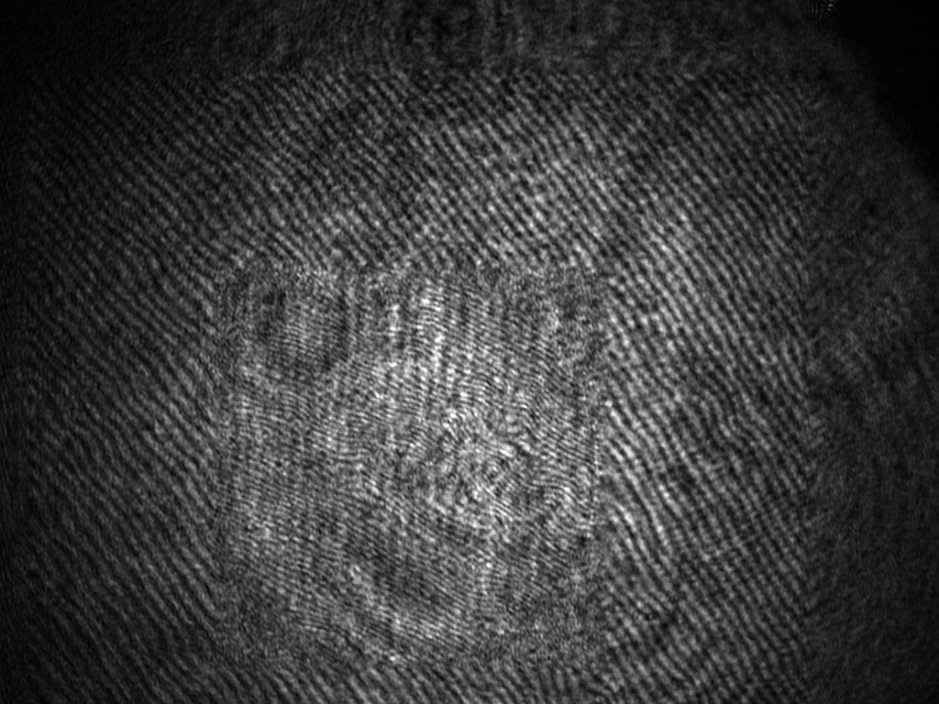
\includegraphics[width=0.5\textwidth]{corrected}
\caption{Interference pattern corrected from the tape distortion}\label{corrected}
\end{figure}
\section{Summary and conclusion}
In this work we used an SLM to create synthetic holograms which we projected on a camera. First we created simple holograms which display a single or multiple points on the screen. We used this holograms to calculate the pixel size of the SLM. Then we also created an hologram to mimic a diffractive lens. We created also more complex holograms of arbitrary images using the Gerchberg-Saxton algorithm. Lastly we used the SLM for adaptive optics application, that is we corrected an optical signal for distortions that we introduced with a piece of transparent tape.

\begin{thebibliography}{99}
\bibitem{grating}
\textsc{Palmer Christopher}, \textit{Diffraction Grating Handbook} (7th edition) Richardson Gratings (2014). 
 \bibitem{camerasite}
 https://www.matrix-vision.com/USB2.0-industrial-camera-mvbluefox.html
 \bibitem{algorithm}
 \textsc{R. W. Gerchberg and W. O. Saxton}, \textit{A practical algorithm for the determination of the phase from image and diffraction plane pictures}, Optik 35, 237 (1972)
 \bibitem{skriptum}
Fortgeschrittenenpraktikum 2, \textit{Excercise FP2-11: Digital holography
}.
\end{thebibliography}
\end{document}
